\documentclass[english, 11pt, a4paper]{article}
\usepackage{notes}
\makeindex
% Uncomment these for a different family of fonts
% \usepackage{cmbright}
% \renewcommand{\sfdefault}{cmss}
% \renewcommand{\familydefault}{\sfdefault}

\newcommand{\thiscoursecode}{[XXXX] (\#\#\#)}
\newcommand{\thiscoursename}{Mål og Integrale Teori}
\newcommand{\thisprof}{Prof. Niels Richard Hansen}
\newcommand{\me}{Rud Faden}
\newcommand{\thisterm}{Blok 2}
\newcommand{\website}{http://kurser.ku.dk}

% Headers
\chead{\thiscoursename \ Course Notes}
\lhead{\thisterm}


%%--------------------------------------------------------------------------
%% Title
%%--------------------------------------------------------------------------
\newcommand{\notefront} {
  \pagenumbering{roman}
  \begin{center}
    \textbf{\Huge{\noun{\thiscoursename}}}{\Huge \par}
    \vspace{0.1em}
    {\noun \thisprof} \ \(\bullet\)  \ {\noun \thisterm} \ \(\bullet\)  \ {\noun {University of Copenhagen}} \\
  \end{center}
}


% Begin Document
\begin{document}

  % Notes front
  \notefront
  % Table of Contents and List of Figures
  \tocandfigures
  % Abstract
  \doabstract{These notes are intended as a resource for myself; past, present, or future students of this course, and anyone interested in the material. The goal is to provide an end-to-end resource that covers all material discussed in the course displayed in an organized manner. If you spot any errors or would like to contribute, please contact me directly.}



% -*- root: ../root.tex -*-
\section{Fundamentels}

\subsection{Paving}

An arbitrary collection of subsets is a  \important{paving}

\subsection{Algebra}
\begin{defn}
A paving \(\mathbb{A}\)  on a set \(X\)  is called an  \important{algebra}
if

\begin{itemize}
  \item \(X\in\mathbb{A}\)
  \item \(A\in\mathbb{A}\Rightarrow A^{c}\in\A\)
  \item \(A,B\in\mathbb{A}\Rightarrow A\cup B\in\A\)
\end{itemize}
\end{defn}
\begin{lem}

If \(\mathbb{A}\)  is an \important{algebra} on \(X\) , then \(\emptyset\in\mathbb{A}\) \end{lem}

\begin{proof}
We know that \(X\)  itself is a member of \(\mathbb{A}\) , and we know that \(\mathbb{A}\)  is is stable under formation of complements. But the complements of \(X\)  is indeed \(\emptyset\) .
\end{proof}

\begin{lem}
If \(\A\)  is an \important{algebra} on \(X\) , is holds that
\[
A,B\in\A\Rightarrow A\cap B\in\A
\]
\end{lem}

\begin{proof}
Take \(A\)  and \(B\)  in \(\A\) . As \(\A\)  is stable under formation of complements, we see that \(A^{c}\)  and \(B^{c}\)  are two \(\A\) -sets. As \(\A\)  is stable under formation of unions, we set that \(A^{c}\cup B^{c}\in\A\) . If we take the complement again, we see that
\[
  A\cap B=(A^{c}\cup B^{c})^{c}\in\A
\]
using {de Morgan's law}
\end{proof}

\begin{lem}
If \(\A\)  is an algebra on \(X\) , it holds that
\[
  A,B\in\A\Rightarrow A\backslash B\in\A
\]
\end{lem}

\begin{proof}
Take \(A\)  and \(B\)  in \(\A\) . As \(\A\)  is stable under the formation of complements, we see that \(B^{c}\)  is in a \(\A\) -set. As \(\A\)  is stable under the formation of intersections, we see that \(A\cap B^{c}\in\A\) . Per definition of the set difference, we have that
\[
A\backslash B=A\cap B^{c}\in\A
\]
\end{proof}

\begin{lem}
If \(\A\)  is an algebra on \(\X\) , and \(\nset{A}\)  are sets in \(\A\) , is holds that
\[
\bigcup_{i=1}^{n}A_{i}\in\A,\:\bigcap_{i=1}^{n}A_{i}\in\A
\]
\end{lem}
\begin{proof}
For \(n=2\)  the claim is included in the definitation of an algebra. If the results is established for \(n-1\)  sets, we have
\[
\bigcup_{i=1}^{n}A_{i}=\left(\bigcup_{i=1}^{n-1}A_{i}\right)\cup A_{n}\in\A
\]
\end{proof}

\subsection{{sigma-algebras}}
\index{sigma algebra}
The concept of algebras does not work under under approximate schemes. Therefore we introduce \(\sigma\)-algrebras.

\begin{defn}
A paving \(\mathbb{E}\)  on a set \(\X\)  is called a \(\sigma\)-algebra if
\begin{itemize}
  \item \(\X\in\es\)
  \item \(A\in\es\Rightarrow A^{c}\in\es\)
  \item \(A_{1},A_{2},\dots\in\es\Rightarrow\bigcup_{i=1}^{\infty}A_{i}\in\es\)
\end{itemize}

\begin{defn}
Lad \(F\) være en abitrær familie a delmænger af \(\X\). Der eksistere en unique \emph{mindste} \(\sigal\) der indeholder alle mængder i \(F\) (\(F\) er ikke selv nødvendigvis en \(\sigal\)). Foreningenmængden af alle \(\sigal\) der indeholder F. Denne \(\sigal\) \(\sigma(F)\) er \(\sigal\)en genereret af F.
\end{defn}
A  \important{measurable space} is a pair \((\X,\es),\)  consisting
of the set \(\X\)  and a \(\sigma\) --algebra \(\es\)  on \(\X\) . We say that
a subset \(A\subset \X\)  is \(\es\) --measurable if \(A\in\es\)
\end{defn}
\begin{lem}
If \(\E\)  is an \(\sigma\)-algebra on \(\X\), the it is also an algebra.
\end{lem}
\begin{proof}
see book page 11.
\end{proof}
\subsection{Borel Sigma algebra} % (fold)
\label{sub:borel_sigma_algebra}
\begin{defn}
  The \important{Borel Sigma algebra}  \(\B\) is the smallest \(\sigal\) generated by the open sets. symboliccally \(\B=\sigma(\os)\)
\end{defn}
\begin{rem}
  As the borel algrebra \(\B\) is a \(\sigal\) which is stabel under the formation of complements, \(\B\) is also the \(sigal\) generated on the closed sets.
\end{rem}
\subsection{Important distributions} % (fold)
\label{sub:important_distrLJibutions}
\begin{table}
  \setlength\extrarowheight{10pt}
  \begin{tabular}{ >{$}l<{$}  >{$}l<{$} | >{$}l<{$}  >{$}l<{$}  }
  \toprule
    \text{Distributions}    & Continues                                                                                                                                                 & Discrete\tabularnewline
    \midrule
    \text{Uniform}          & \displaystyle\frac{1}{\beta}, \text{ for } x\in(\alpha,\alpha+\beta)                                                                                      & \text{Bionomial} & \displaystyle \begin{pmatrix} n \\ x\end{pmatrix}p^x(1-p)^{n-x} \tabularnewline
    \text{Exponential}      &\displaystyle \frac{1}{\beta}e^{-x/\beta}                                                                                                                  & \text{H-gemometric}& \displaystyle \begin{pmatrix}N_1 \\ x \end{pmatrix}\begin{pmatrix}N-N_1 \\ n-x \end{pmatrix}\Biggm/\begin{pmatrix} N \\N \end{pmatrix} \tabularnewline
    \text{Cauchy}           & \displaystyle\frac{1}{\pi(1+x^2)}                                                                                                                         & \text{Poisson} & \displaystyle\frac{\lambda^x}{x!}e^{-\lambda}\tabularnewline
    \text{Normal}           & \displaystyle\frac{1}{\sqrt{2\pi}}e^{-(x-\xi)^2/2\sigma^2}                                                                                                & &\tabularnewline
    \text{Gamma } \Gamma & \displaystyle\frac{1}{\beta^\lambda\Gamma(\lambda)}x^{1-\lambda}e^{-x/\beta}                                                                                 & &\tabularnewline
    \text{Beta}             & \displaystyle\frac{1}{\lambda_1,\lambda_2}x^{\lambda_1-1}(1-)^{\lambda_2-1}                                                                               & &\tabularnewline
    \text{F}                & \displaystyle\frac{\lambda_1^{\lambda_1}\lambda_2^{\lambda_2}}{B(\lambda_1,\lambda_2)}\frac{x^{\lambda_1-1}}{(\lambda_1x+\lambda_2)^{\lambda_+\lambda_2}} & &\tabularnewline
    \text{T}                & \displaystyle\frac{1}{\sqrt{2\lambda}B(\lambda,\frac{1}{2})}\frac{1}{\left(1+\frac{x^2}{2\lambda}\right)^{\lambda+1/2}}                                   & &\tabularnewline

    \bottomrule
  \end{tabular}
  \caption{distributions}
  \label{tbl:label}
\end{table}

% subsection important_distributions (end)
% subsubsection borel_sigma_algebra (end)
% -*- root: ../root.tex -*-
\section[Lecture 1]{Measures} % (fold)
\label{sec:lecture_1}
\begin{defn}
\index{Borel \(\sigma\)-algebraen}Borel \(\sigma\)-algebraen \(\B_k\) på \(\R_k\) er \(\sigal\) frembragt på de åbne mængder \(\os_k\)
\end{defn}
% \begin{exercise}
% Afgør om det er er borel mængder
% \begin{enumerate}[label=(\arabic*)]
%   \item \((\R,\B)\) er et målbart rum.
% \[
%   a,b \Rightarrow A\cup B^c\in\B
% \]
% \item Hvis \(B\subseteq\) er en endelig mængde, så gælder at \(B\in\B\)
% \item \(\{x\}\in\B\) for alle \(x\in\R\)
% \item Hvis \(B\subseteq\R\) er en tællig mængde, så gælder det at \(B\in\B\).
% \item Hvis \(B\subseteq\B\) er overtællig mængde med tællig \(B^c\), så \(B\in\B\)
% \end{enumerate}
% \end{exercise}
% \begin{solution}
% Løsning på overstående
% \begin{enumerate}[label=(\arabic*)]
%   \item Sandt: En \(\sigal\) er \important{stabil} over for  \important{endelige} og  \important{tællige} mængdeoperation
%   \item Falsk: \(\B\ne\pow(\R)\) så findes \(B\in \pow(\R)\) så \(B\in\B\). Så \(\R=B\union B^c\). So if \(B\) er overtællig, så er \(B^c\) også overtællig. Derved er findes der et \(B\notin\B\)
%   \item Sandt:\(\{x\}\) er endelig og \(\B\) indeholder alle \important{endelige!mængder}
%   \item \(B\bigcup_{x\in B}\{x\}\), som er tællig, hvis \(B\) er tællig
%   \item Hvis \(B\) er overtællig, \(B^c\) er tællig, så \(B^c\in\B\), så \(B=(B^c)^c\in B\) (\(B\) er stabil under komplimenter), så \(B\in\B\)
% \end{enumerate}
% \end{solution}

\(\B=\sigma(\os)\), dvs, den mindste \(sigal\) der indeholder \(\os\). F.eks.
\begin{itemize}
  \item De endelige mængder
  \item De åbne kasser \(\I^k\)
  \item De åbne kasser med rationelle hjørner
  \item For \(k=1\), intervaller af formen \((-\infty,b_1],\ldots,\times(-\infty,b_i] \)
\end{itemize}
Lad \(\X\) være en mængde og lad \(\es=\sigma(\X)\), så kaldes \((\X,\es)\) et målbart rum.
\begin{defn}
Et mål \(\mu\) på \((\X,\es)\) er en funktion på \(\es\) som opfylder
\begin{itemize}
  \item \(\mu(A_n)\in[0,\infty]\)
  \item \(\mu(\emptyset)=0\)
  \item \(\mu\left(\bigcup_{n=1}^\infty A_n\right)=\sum_{n=1}^\infty \mu(A_n)\)
\end{itemize}
\end{defn}
\begin{exmp}
Arealet på \((b_i-a_1)(b_2-a_2)\)\tabularnewline
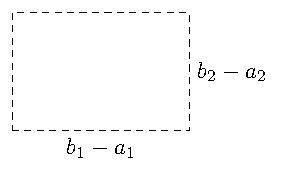
\includegraphics{fig/box.pdf}
\end{exmp}

\subsection{lebesgue målet} % (fold)
\label{sub:lebesgue_m_let}
\begin{defn}
\[
  m_k((a_1,b_1)\times(a_2,b_2)\times\ldots\times(a_k,b_k))=\prod_{i=1}^k(a_i,b_i)
\]
\end{defn}
\subsection{Intergation with respect to a measure} % (fold)
\label{sub:intergation_with_respect_to_a_measure}
When we write something like \(\dif x\) in a integral \(\int f(x) \dif x\) we mean the infinitesimal interval starting at \(x\). So \(\dif x\) tell us 3 things. (i) which variable we are dealing with (ii) the value of that variable, and (iii) the length of a infinitesimal at that value. When we integrate with respect to a measure \(\mu\), we write \(\mu(\dif x)\), which is short hand for \(\mu(x,x+\dif x)\). That is the measure of a infinitesimal change in interval starting at \(x\). So in a intergral
\[
  \int f(x) \mu(\dif x)
\]
\(f(x)\) is the height and \(\mu(\dif x)\) is the lenght of the infinitisimal area \(f(x) \mu(\dif x)\)
% subsection intergation_with_respect_to_a_measure (end)
% \begin{exercise}
% Afgør om følgende er sandt eller falsk
% \begin{enumerate}
%   \item hvis \(A\subseteq B\) med \(\mu(A)=0\) og \(B\subseteq A\) så \(B\in \B\)
%   \item \(\mu(\R)=\lim_{n \rightarrow \infty}\mu[-n,n]\)
%   \item \(\mu(\{0\})=\lim_{n \rightarrow \infty}(\left[-n^{-1},n^{-1}\right])\)
%   \end{enumerate}
% \end{exercise}

% \begin{solution}
% Løsninger på overstående
% \begin{enumerate}
%   \item  Falsk: Der findes (for f.eks. lebesgue målet) ikke målige nul mængder. Dvs. \(B\subseteq A\), hvor \(\mu(A)=0\), og \(B\in\R\)
% \item Sandt: \(\R=\bigcup_{n\in\N}[-n,n]\) og \(\left[-n,n\right]\) vokser opad (dvs. \([-1,1]\subseteq[-2,2]\subseteq\ldots\subseteq [-n,n]\). Da målet er opad kontinuert, så er \(\mu\bigcup_n[-n,n]=\lim_{n \rightarrow \infty}\mu\bigcup_n[-n,n]\)
% \item Falsk: \(\{0\}=\bigcap_{n\in\N}\left[-n^{-1},n^{-1}\right]\). Tag f.eks. tællemålet \(\mu=\tau\). \(\tau(\{0\})=1\) men \\ \(\tau\left[-n^{-1},n^{-1}\right]=\infty\)
% \end{enumerate}
% \end{solution}

% -*- root: ../root.tex -*-
\section[Lecture 2]{The Uniquness  Thoerem} % (fold)
\label{sec:lecture_2}

\subsubsection*{The Uniqueness Theorem} % (fold)
\label{ssub:the_uniqueness_theorem}
The problem is that we would like to say something about then two measures on the same measurable space \(\X,\E\) on ``many'' sets (e.g. the the power set). E.i, when \(\mu(A)=\upsilon(A)\).

We cannot check all sets in \(\E\). So we would like to say something about how many sets we need to check to astablish that \(\mu(A)=\upsilon(A)\) for all \(A\in\E\)?

For some paving \(\D\) and a \(\E=\sigma(\D)\) and two measures \(\mu\) and \(\upsilon\) we want to show that if \(\mu(D)=\upsilon(D)\, \forall \, D\in \D\) then it also holds that \(\mu(A)=\upsilon(A)\, \forall \, A\in \E\) trick is to:
\begin{enumerate}
  \item Show that \(\mu(D)=\upsilon(D)\, \forall \, D\in\D\)
  \item Then construct a set \(\sH=\{A\in\E\mid \mu(A)=\upsilon(A)\}\supset\D\)
  \item Then show that \(\sH=\E\)
\end{enumerate}

The last part is however not easy unless we can show that \(\sH\) is a \(\sigal\). So instead we make a loser requirement on \(\sH\) and then try to show that \(\sH=\E\) given some stronger requirements on \(\D\) than just being a generator for the \(\sigal\).
\begin{defn}
A paving \(\sH\) os a set \(\X\) is a \important{Dynkin class} if
\begin{enumerate}
  \item \(\X\in\sH\) (the same as \(\sigma\)-algebra)
  \item \(A,B\in\sH,\, A\subset B \Rightarrow B\setminus A\in \sH\) (stronger than the \(\sigma\)-algebra but as \(\X\setminus A=A^c\) then it is also stable under complements)
  \item \(\nset{A}\in\sH,\, \nsubseti{A} \Rightarrow \bigcup_{n=1}^\infty A_n\) (looser than \(\sigma\)-algebra)
\end{enumerate}
\end{defn}
To show that a Dynkins class is af \(\sigma\)-algebra and vice-versa we need to lemmas
\begin{lem}
if \(\A\) is an algebra it holds that
\[
  A,B\in\A \Rightarrow A\setminus B\in \A
\]
\end{lem}
\begin{lem}
If \(\E\) is a \(\sigma\)-algebra it is also an algebra
\end{lem}
So the property that \(A,B\in\A \Rightarrow A\setminus B\in \A \) also holds for a \(\sigma\)-algebra.

We then introduce a new lemma that states \(\E=\sH\) and that \(\sH=\E\).
\begin{lem}
 If \(\E\) is a \(\sigma\)-algebra, then \(\E\) is also a Dynkins Class. If \(\sH\) is a Dynkins class which is stable under intersections, then \(\sH\) is a \(\sigma\)-algebra.
 \end{lem}
 \begin{proof}
 The first part follows easlialy. (1) is the same for both (2) follows from the two lemmas stating that if \( A,B\in\A \Rightarrow A\setminus B\in \A\) holds for a \(\sigma\)-algebra. (3) holds, as a \(\sigma\)-algebra is stable under all types of unions, also unions of increasing sets. To show that \(\sH\) which is \(cap\)-stabe  is a \(\sigma\)-algebra we first note that a DC which is stable under \(\cap\) is also stable  under finite \(\cup\): if \(A,B\in\sH\) then
 \[
   A\cup B=(A^c\cap B^c)^c\in\sH
 \]
 if \(\nseti{A}\in\sH\), we let
 \[
   B_n=A_1\cup\ldots\cup A_n
 \]
 As a \(\cap\)-stable DC is stable under finite unions, then \(B_n\in\sH\). And as \(\nsubseti{B}\) we have that \(\bigcup_{n=1}^\infty B_n\in\sH\). But
 \[
   \bigcup_{n=1}^\infty B_n=\bigcup_{n=1}^\infty A_n
 \]
 \end{proof}
So if a DC \(\sH\) is \(\cap\)-stable it is in fact a \(\sigma\)-algebra.
\begin{rem}
If \((\sH_i)_{i\in I}\) is a family of DC, the intersection \(\bigcap_{i\in I}\sH_i\) is also a DC
\end{rem}
\begin{rem}
A DC generated by \(\D\) is the smallest DC containg all the elements of \(\D\)
\end{rem}
\begin{lem}[\index{Dynkins lemma}Dynkins lemma]
Let \(\D\subset\sH\subset\E\) be pavings on the set \(\X\), and assume that \(\E=\sigma(\D)\). If \(\D\) is \(\cap\)-stable, and if \(\sH\) is a DC, then \(\sH=\E\).
\end{lem}
\begin{proof}
Let \(\K\) be the smallest DC containing \(\D\). Then
\[
  \D\subset\K\subset\sH\subset\E
\]
The proof is to show that \(\K\) is \(\cap\)-stabel. If this is true, then it follows from above lemma that \(\K\) is a \(\sigma\)-algebra. As \(\E\) is the smallest \(\sigma\)-algebra containing \(\D\) and \(\K\) is a \(\sigma\)-algebra contaning \(\D\) than it must be true that \(\K=\E\). As \(\sH\) is squezzed between \(\K\) and \(\E\) then \(\sH=\E\). E.i. \(\sH\) is a \(\sigma\)-algebra.

The proof follows as
\begin{enumerate}
  \item Show that \(\K\) is \(\cap\)-stabel

for each \(A\in\K\), introduce a new paving
\[
  \K_A=\left\{ B\in\K\mid A\cap B\in \K\right\}
\]
\(\K_A\) is a DC as
\begin{enumerate}[label=(\alph*)]
  \item \(\X\in\K_A\) as \(A\cap\X \Rightarrow A\subset\D\subset\K\). As \(\K_A\) is the intersection of all elements of \(\K\) and \(\X\) is a element of \(\K\)
  \item \(\tilde{A},B,\tilde{A}\subset B \Rightarrow B\setminus\tilde{A}\in\K_A\). Then \(\tilde{A}\cap A, B\cap A\in \K\) with \(\tilde{A}\cap A\subset B\cap A \). So
  \[
    (B\setminus\tilde{A})\cap A=\underbrace{(B\cap A)}_{\in\K}\setminus \underbrace{(\tilde{A}\cap A)}_{\in\K}
  \]
So \(B\setminus\tilde{A}\in\K\)
\item \(\nseti{B}\in\K_A,\, \nsubseti{B} \Rightarrow \bigcup_{n=1}^\infty B_n \in\K_A\)
\[
  A\cap \bigcup_{n=1}^\infty B_n=\bigcup_{n=1}^\infty\underbrace{(A\cap B_n)}_{\in\K}
\]
as \(\K\) is a DC. Further \(\nsubseti{A\cap B}\), so \(\bigcup_{n=1}^\infty A\cap B_n\in\K_A\)
\end{enumerate}
\end{enumerate}
\begin{enumerate}[resume]
  \item Note that \(\D\subset\K_A\subset\K\) and for \(A,B\in\D\), then \(A\cap B\in\D\subset \K\) which can given the definition of \(\K_A\) this can be reformulated as: if \(A\in\D\), then \(\D\subset\K_A\) we must have that \(\K_A=\K\). \(\K\) is the smallest DC that contains \(\D\) and \(\D\subset\K_A\), then \(\K_A=\K\). And a \(\K_A\) is defined by the intersections of \(\K\) then \(\K\) is \(\cap\)-stabel.
\end{enumerate}
\begin{figure}[htbp]
  \centering
  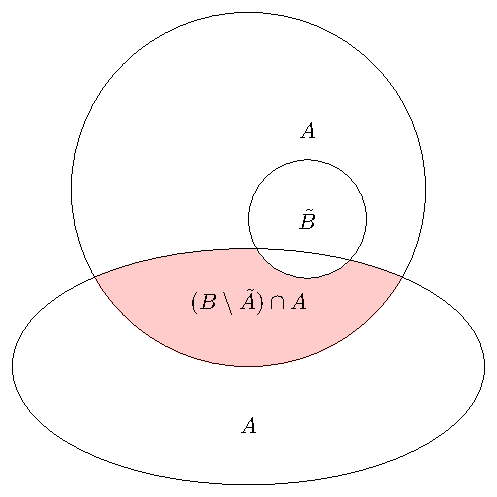
\includegraphics[width=0.5\textwidth]{fig/intersec.pdf}
  \caption{The \((B\setminus\tilde{A})\cap A\) }
  \label{fig:label}
\end{figure}
\end{proof}
Using the above we can then prove the \important{uniqueness theorem for!probability measures}. The steps are as follows
\begin{enumerate}
  \item Let \(\upsilon,\mu\) be two measures of probability on a measurable space, and assume that \(\E=\sigma(\D)\) and that
  \[
    \mu(D)=\upsilon(D)
  \]
if \(\D\) is \(\cap\)-stabel, then \(\mu=\upsilon\).
  \item contruct a paving where the two measures are equal
  \[
    \sH=\{F\in\E\mid \mu(F)=\upsilon(F)\}
  \]
  and show that \(\sH\) is a DC. This can be done with Dynkins lemma, which requires that
  \begin{enumerate}
    \item That \(\D\) is \(\cap\)-stabel follows by the theorem
    \item establish that \(\D\subset\sH\subset\E\). But this clearly follows from the contruction of \(\sH\)
    \item Then all we need to show is that \(\sH\) is a DC
  \end{enumerate}
  To show that \(\sH\) is a DC we note that
  \begin{itemize}
    \item As \(\mu,\upsilon\) are probability measures, then clearly \(\X\in\sH\).
    \item If \(A\subset B\) are two \(\sH\) sets, then
    \[
      \mu(B\setminus A)=\mu(B)-\mu(A)=\upsilon(B-\upsilon(A))=\upsilon(B\setminus A)
    \],
    so \(B\setminus A\in\sH\)
    \item If \(\nsubseti{F}\in\sH\), then
    \[
      \mu\left(\bigcup_{n=1}^\infty F_n\right)=\lim_{n \rightarrow\infty} \mu(F_n)=\lim_{n \rightarrow\infty}\upsilon(F_n)=\upsilon\left(\bigcup_{n=1}^\infty F_n\right)
    \],
    then \(\bigcup_{n=1}^\infty F_n\in\sH\)


  \end{itemize}

\end{enumerate}
\subsection{Product Algebra} % (fold)
\label{ssub:product_algebra}
Looks a \(\sigma\)-algebra generated by several maps. That is, if you have many measurable maps and you take the cartisan product, will the product then still be measurable.
% subsubsection product_algebra (end)
\subsection{Measurability of intergrals} % (fold)
\label{sub:measurability_of_intergrals}
Examine under what conditions a integral is measurable
% subsection measurability_of_intergrals (end)
\subsection{Measurable maps} % (fold)
\label{sub:measurable_maps}
\begin{defn}\label{measurable_map}
Lad \(\X,\E\) and \(\Y,\K\) be two measurable spaces, and let \(f:\X \rightarrow \Y\) be a map. We say that \(f\) is \important{measurable} if
\[
  f^{-1}(B)\in\E \text{ for all } B\in\K
\]
\end{defn}
\begin{rem}
We say that a \(f\) is \(\E-\K\) measurable if it satifies above
\end{rem}
\begin{rem}
If there is no confusion about which algebra to use, we say that either \(f\) is \(\E\)-measurable if the \(\sigma\)-algebra \(\Y\) is fixed and the only choice of confusion is the \(\sigma\)-algebra on \(\X\). Similary we may say that that \(f\) is \(\K\) measurable if \(\X\) is fixed, and the only possible confusion is the choice of \(\sigma\)-algebra on \(\Y\)
\end{rem}
Often we cannot check all the sets in the \(\sigma\)-algebra as many of them are not acceseable for direct description. Luckly we only have to check the condition given in \cref{measurable_map} on the generator for for the \(\sigma\)-algebra.

\begin{lem}
Let \((\X,\E)\) and \(\Y,\K\) be two measurable spaces, and let \(f:\X \rightarrow \Y\) be a map. Let \(\D\) be a paving on \(\Y\) and assume that \(\K=\sigma(\D)\) . If
\[
  f^{-1}(D)\in\E\, \forall\, D\in\D,
\]
then \(f\) is \(\E-\K\)-measurable
\end{lem}
% subsection measurable_maps (end)
\subsection{Product measures} % (fold)
\label{ssub:product_measures}
Thw product of two finite measures \(\mu\otimes\upsilon\) is agian a measure. Especially: the product of two probability measures is agian a probability measure.

\begin{them}
Let \((\X,\E, \mu)\) and \(\Y,\K, \upsilon\) be \(\sigma\)-finite spaces. Then there is a unique measure \(\mu\otimes\upsilon\) on the product space \(\X\times\Y, \E\otimes\K\) satesfying that
\[
  \mu\otimes\upsilon(A\times B)=\mu(A)\upsilon(B)\quad A\in\E,B\in\K
\]

\end{them}
% -*- root: ../root.tex -*-
% subsubsection product_measures (end)
\section{Lecture 3} % (fold)
\label{sec:lecture_3}
\subsection{Integration of a product measure} % (fold)
\label{sub:integration_of_a_product_measure}
\begin{them}[Tonelli\index{Tonelli}]
Let \((\X,\E,\mu)\) and \((\mathcal{Y},\K,\upsilon)\) be two \(\sigma\)-finite measurable spaces and let \(d\in \mathcal{M}^+(\X\times\mathcal{Y},\E\otimes\K)\).It holds that
\[
  \int fd\mu\otimes \upsilon=\int\left(\int f(y,x)d\mu(y)\right)d\upsilon(x)
\]

\end{them}
% subsection integration_of_a_product_measure (end)
% section lecture_3 (end)
% section lecture_2 (end)
\printindex

\end{document}
